\documentclass[]{article}
\usepackage{lmodern}
\usepackage{amssymb,amsmath}
\usepackage{ifxetex,ifluatex}
\usepackage{fixltx2e} % provides \textsubscript
\ifnum 0\ifxetex 1\fi\ifluatex 1\fi=0 % if pdftex
  \usepackage[T1]{fontenc}
  \usepackage[utf8]{inputenc}
\else % if luatex or xelatex
  \ifxetex
    \usepackage{mathspec}
  \else
    \usepackage{fontspec}
  \fi
  \defaultfontfeatures{Ligatures=TeX,Scale=MatchLowercase}
  \newcommand{\euro}{€}
\fi
% use upquote if available, for straight quotes in verbatim environments
\IfFileExists{upquote.sty}{\usepackage{upquote}}{}
% use microtype if available
\IfFileExists{microtype.sty}{%
\usepackage{microtype}
\UseMicrotypeSet[protrusion]{basicmath} % disable protrusion for tt fonts
}{}
\usepackage[margin=1in]{geometry}
\usepackage{hyperref}
\PassOptionsToPackage{usenames,dvipsnames}{color} % color is loaded by hyperref
\hypersetup{unicode=true,
            pdftitle={Week 2},
            pdfauthor={Daniel Brooks (daniel.brooks@spsmail.cuny.edu), Daniel Fanelli (daniel.fanelli@spsmail.cuny.edu), Christopher Fenton (christopher.fenton@spsmail.cuny.edu), James Hamski (james.hamski@spsmail.cuny.edu), Youqing Xiang (youqing.xiang@spsmail.cuny.edu)},
            pdfborder={0 0 0},
            breaklinks=true}
\urlstyle{same}  % don't use monospace font for urls
\usepackage{color}
\usepackage{fancyvrb}
\newcommand{\VerbBar}{|}
\newcommand{\VERB}{\Verb[commandchars=\\\{\}]}
\DefineVerbatimEnvironment{Highlighting}{Verbatim}{commandchars=\\\{\}}
% Add ',fontsize=\small' for more characters per line
\usepackage{framed}
\definecolor{shadecolor}{RGB}{248,248,248}
\newenvironment{Shaded}{\begin{snugshade}}{\end{snugshade}}
\newcommand{\KeywordTok}[1]{\textcolor[rgb]{0.13,0.29,0.53}{\textbf{{#1}}}}
\newcommand{\DataTypeTok}[1]{\textcolor[rgb]{0.13,0.29,0.53}{{#1}}}
\newcommand{\DecValTok}[1]{\textcolor[rgb]{0.00,0.00,0.81}{{#1}}}
\newcommand{\BaseNTok}[1]{\textcolor[rgb]{0.00,0.00,0.81}{{#1}}}
\newcommand{\FloatTok}[1]{\textcolor[rgb]{0.00,0.00,0.81}{{#1}}}
\newcommand{\ConstantTok}[1]{\textcolor[rgb]{0.00,0.00,0.00}{{#1}}}
\newcommand{\CharTok}[1]{\textcolor[rgb]{0.31,0.60,0.02}{{#1}}}
\newcommand{\SpecialCharTok}[1]{\textcolor[rgb]{0.00,0.00,0.00}{{#1}}}
\newcommand{\StringTok}[1]{\textcolor[rgb]{0.31,0.60,0.02}{{#1}}}
\newcommand{\VerbatimStringTok}[1]{\textcolor[rgb]{0.31,0.60,0.02}{{#1}}}
\newcommand{\SpecialStringTok}[1]{\textcolor[rgb]{0.31,0.60,0.02}{{#1}}}
\newcommand{\ImportTok}[1]{{#1}}
\newcommand{\CommentTok}[1]{\textcolor[rgb]{0.56,0.35,0.01}{\textit{{#1}}}}
\newcommand{\DocumentationTok}[1]{\textcolor[rgb]{0.56,0.35,0.01}{\textbf{\textit{{#1}}}}}
\newcommand{\AnnotationTok}[1]{\textcolor[rgb]{0.56,0.35,0.01}{\textbf{\textit{{#1}}}}}
\newcommand{\CommentVarTok}[1]{\textcolor[rgb]{0.56,0.35,0.01}{\textbf{\textit{{#1}}}}}
\newcommand{\OtherTok}[1]{\textcolor[rgb]{0.56,0.35,0.01}{{#1}}}
\newcommand{\FunctionTok}[1]{\textcolor[rgb]{0.00,0.00,0.00}{{#1}}}
\newcommand{\VariableTok}[1]{\textcolor[rgb]{0.00,0.00,0.00}{{#1}}}
\newcommand{\ControlFlowTok}[1]{\textcolor[rgb]{0.13,0.29,0.53}{\textbf{{#1}}}}
\newcommand{\OperatorTok}[1]{\textcolor[rgb]{0.81,0.36,0.00}{\textbf{{#1}}}}
\newcommand{\BuiltInTok}[1]{{#1}}
\newcommand{\ExtensionTok}[1]{{#1}}
\newcommand{\PreprocessorTok}[1]{\textcolor[rgb]{0.56,0.35,0.01}{\textit{{#1}}}}
\newcommand{\AttributeTok}[1]{\textcolor[rgb]{0.77,0.63,0.00}{{#1}}}
\newcommand{\RegionMarkerTok}[1]{{#1}}
\newcommand{\InformationTok}[1]{\textcolor[rgb]{0.56,0.35,0.01}{\textbf{\textit{{#1}}}}}
\newcommand{\WarningTok}[1]{\textcolor[rgb]{0.56,0.35,0.01}{\textbf{\textit{{#1}}}}}
\newcommand{\AlertTok}[1]{\textcolor[rgb]{0.94,0.16,0.16}{{#1}}}
\newcommand{\ErrorTok}[1]{\textcolor[rgb]{0.64,0.00,0.00}{\textbf{{#1}}}}
\newcommand{\NormalTok}[1]{{#1}}
\usepackage{graphicx,grffile}
\makeatletter
\def\maxwidth{\ifdim\Gin@nat@width>\linewidth\linewidth\else\Gin@nat@width\fi}
\def\maxheight{\ifdim\Gin@nat@height>\textheight\textheight\else\Gin@nat@height\fi}
\makeatother
% Scale images if necessary, so that they will not overflow the page
% margins by default, and it is still possible to overwrite the defaults
% using explicit options in \includegraphics[width, height, ...]{}
\setkeys{Gin}{width=\maxwidth,height=\maxheight,keepaspectratio}
\setlength{\parindent}{0pt}
\setlength{\parskip}{6pt plus 2pt minus 1pt}
\setlength{\emergencystretch}{3em}  % prevent overfull lines
\providecommand{\tightlist}{%
  \setlength{\itemsep}{0pt}\setlength{\parskip}{0pt}}
\setcounter{secnumdepth}{5}

%%% Use protect on footnotes to avoid problems with footnotes in titles
\let\rmarkdownfootnote\footnote%
\def\footnote{\protect\rmarkdownfootnote}

%%% Change title format to be more compact
\usepackage{titling}

% Create subtitle command for use in maketitle
\newcommand{\subtitle}[1]{
  \posttitle{
    \begin{center}\large#1\end{center}
    }
}

\setlength{\droptitle}{-2em}
  \title{Week 2}
  \pretitle{\vspace{\droptitle}\centering\huge}
  \posttitle{\par}
  \author{Daniel Brooks
(\href{mailto:daniel.brooks@spsmail.cuny.edu}{\nolinkurl{daniel.brooks@spsmail.cuny.edu}}),
Daniel Fanelli
(\href{mailto:daniel.fanelli@spsmail.cuny.edu}{\nolinkurl{daniel.fanelli@spsmail.cuny.edu}}),
Christopher Fenton
(\href{mailto:christopher.fenton@spsmail.cuny.edu}{\nolinkurl{christopher.fenton@spsmail.cuny.edu}}),
James Hamski
(\href{mailto:james.hamski@spsmail.cuny.edu}{\nolinkurl{james.hamski@spsmail.cuny.edu}}),
Youqing Xiang
(\href{mailto:youqing.xiang@spsmail.cuny.edu}{\nolinkurl{youqing.xiang@spsmail.cuny.edu}})}
  \preauthor{\centering\large\emph}
  \postauthor{\par}
  \predate{\centering\large\emph}
  \postdate{\par}
  \date{6/26/2016}



% Redefines (sub)paragraphs to behave more like sections
\ifx\paragraph\undefined\else
\let\oldparagraph\paragraph
\renewcommand{\paragraph}[1]{\oldparagraph{#1}\mbox{}}
\fi
\ifx\subparagraph\undefined\else
\let\oldsubparagraph\subparagraph
\renewcommand{\subparagraph}[1]{\oldsubparagraph{#1}\mbox{}}
\fi

\begin{document}
\maketitle

\subsubsection{1. Download/read the classification output data
set}\label{downloadread-the-classification-output-data-set}

\begin{Shaded}
\begin{Highlighting}[]
\NormalTok{data <-}\StringTok{ }\KeywordTok{read.csv}\NormalTok{(}\StringTok{'classification-output-data.csv'}\NormalTok{)}
\KeywordTok{summary}\NormalTok{(data)}
\end{Highlighting}
\end{Shaded}

\begin{verbatim}
##     pregnant         glucose        diastolic        skinfold   
##  Min.   : 0.000   Min.   : 57.0   Min.   : 38.0   Min.   : 0.0  
##  1st Qu.: 1.000   1st Qu.: 99.0   1st Qu.: 64.0   1st Qu.: 0.0  
##  Median : 3.000   Median :112.0   Median : 70.0   Median :22.0  
##  Mean   : 3.862   Mean   :118.3   Mean   : 71.7   Mean   :19.8  
##  3rd Qu.: 6.000   3rd Qu.:136.0   3rd Qu.: 78.0   3rd Qu.:32.0  
##  Max.   :15.000   Max.   :197.0   Max.   :104.0   Max.   :54.0  
##     insulin            bmi           pedigree           age       
##  Min.   :  0.00   Min.   :19.40   Min.   :0.0850   Min.   :21.00  
##  1st Qu.:  0.00   1st Qu.:26.30   1st Qu.:0.2570   1st Qu.:24.00  
##  Median :  0.00   Median :31.60   Median :0.3910   Median :30.00  
##  Mean   : 63.77   Mean   :31.58   Mean   :0.4496   Mean   :33.31  
##  3rd Qu.:105.00   3rd Qu.:36.00   3rd Qu.:0.5800   3rd Qu.:41.00  
##  Max.   :543.00   Max.   :50.00   Max.   :2.2880   Max.   :67.00  
##      class         scored.class    scored.probability
##  Min.   :0.0000   Min.   :0.0000   Min.   :0.02323   
##  1st Qu.:0.0000   1st Qu.:0.0000   1st Qu.:0.11702   
##  Median :0.0000   Median :0.0000   Median :0.23999   
##  Mean   :0.3149   Mean   :0.1768   Mean   :0.30373   
##  3rd Qu.:1.0000   3rd Qu.:0.0000   3rd Qu.:0.43093   
##  Max.   :1.0000   Max.   :1.0000   Max.   :0.94633
\end{verbatim}

\subsubsection{2. Use the table() function to get the raw confusion
matrix for this scored
dataset}\label{use-the-table-function-to-get-the-raw-confusion-matrix-for-this-scored-dataset}

\begin{Shaded}
\begin{Highlighting}[]
\NormalTok{cf <-}\StringTok{ }\KeywordTok{table}\NormalTok{(data[,}\DecValTok{9}\NormalTok{:}\DecValTok{10}\NormalTok{])}
\NormalTok{cf}
\end{Highlighting}
\end{Shaded}

\begin{verbatim}
##      scored.class
## class   0   1
##     0 119   5
##     1  30  27
\end{verbatim}

Explain:

\begin{itemize}
\tightlist
\item
  column (scored.class): the predicted class
\item
  row (class): the actual class
\item
  class = 0 and scored.class = 0: there are 119 observations which are
  predicted correctly with class 0
\item
  class = 0 and scored.class = 1: there are 5 observations which are
  class 0 but are predicted with class 1
\item
  class = 1 and scored.class = 0: there are 30 obervations which are
  class 1 but are predicted with class 0
\item
  class = 1 and scored.class = 1: there ae 27 obervations which are
  correctly predicted with class 1.
\end{itemize}

\subsubsection{3. Write a function that takes the data set as a
dataframe, with actual and predicted classifications identified, and
returns the accuracy of the
predictions.}\label{write-a-function-that-takes-the-data-set-as-a-dataframe-with-actual-and-predicted-classifications-identified-and-returns-the-accuracy-of-the-predictions.}

\begin{Shaded}
\begin{Highlighting}[]
\NormalTok{my_accuracy <-}\StringTok{ }\NormalTok{function(data) \{}
  \NormalTok{cf <-}\StringTok{ }\KeywordTok{table}\NormalTok{(data[,}\DecValTok{9}\NormalTok{:}\DecValTok{10}\NormalTok{])}
  \NormalTok{cf <-}\StringTok{ }\KeywordTok{as.data.frame}\NormalTok{(cf)}
  \NormalTok{accuracy <-}\StringTok{ }\NormalTok{(cf$Freq[}\DecValTok{1}\NormalTok{] +}\StringTok{ }\NormalTok{cf$Freq[}\DecValTok{4}\NormalTok{])/}\KeywordTok{sum}\NormalTok{(cf$Freq)}
  \KeywordTok{return}\NormalTok{(accuracy)}
\NormalTok{\}}
\end{Highlighting}
\end{Shaded}

\subsubsection{4. Write a function that takes the data set as a
dataframe, with actual and predicted classifications identified, and
returns the classification error rate of the
predictions.}\label{write-a-function-that-takes-the-data-set-as-a-dataframe-with-actual-and-predicted-classifications-identified-and-returns-the-classification-error-rate-of-the-predictions.}

\begin{Shaded}
\begin{Highlighting}[]
\NormalTok{my_error <-}\StringTok{ }\NormalTok{function(data) \{}
  \NormalTok{cf <-}\StringTok{ }\KeywordTok{table}\NormalTok{(data[,}\DecValTok{9}\NormalTok{:}\DecValTok{10}\NormalTok{])}
  \NormalTok{cf <-}\StringTok{ }\KeywordTok{as.data.frame}\NormalTok{(cf)}
  \NormalTok{error <-}\StringTok{ }\NormalTok{(cf$Freq[}\DecValTok{2}\NormalTok{] +}\StringTok{ }\NormalTok{cf$Freq[}\DecValTok{3}\NormalTok{])/}\KeywordTok{sum}\NormalTok{(cf$Freq)}
  \KeywordTok{return}\NormalTok{(error)}
\NormalTok{\}}
\end{Highlighting}
\end{Shaded}

\subsubsection{5. Write a function that takes the data set as a
dataframe, with actual and predicted classifications identified, and
returns the precision of the
predictions.}\label{write-a-function-that-takes-the-data-set-as-a-dataframe-with-actual-and-predicted-classifications-identified-and-returns-the-precision-of-the-predictions.}

\begin{Shaded}
\begin{Highlighting}[]
\NormalTok{my_precision <-}\StringTok{ }\NormalTok{function(data) \{}
  \NormalTok{cf <-}\StringTok{ }\KeywordTok{table}\NormalTok{(data[,}\DecValTok{9}\NormalTok{:}\DecValTok{10}\NormalTok{])}
  \NormalTok{cf <-}\StringTok{ }\KeywordTok{as.data.frame}\NormalTok{(cf)}
  \NormalTok{precision <-}\StringTok{ }\NormalTok{cf$Freq[}\DecValTok{4}\NormalTok{]/(cf$Freq[}\DecValTok{4}\NormalTok{] +}\StringTok{ }\NormalTok{cf$Freq[}\DecValTok{3}\NormalTok{])}
  \KeywordTok{return}\NormalTok{(precision)}
\NormalTok{\}}
\end{Highlighting}
\end{Shaded}

\subsubsection{6. Write a function that takes the data set as a
dataframe, with actual and predicted classifications identified, and
returns the sensitivity of the predictions. Sensitivity is also known as
recall.}\label{write-a-function-that-takes-the-data-set-as-a-dataframe-with-actual-and-predicted-classifications-identified-and-returns-the-sensitivity-of-the-predictions.-sensitivity-is-also-known-as-recall.}

\begin{Shaded}
\begin{Highlighting}[]
\NormalTok{my_sensitivity <-}\StringTok{ }\NormalTok{function(data) \{}
  \NormalTok{cf <-}\StringTok{ }\KeywordTok{table}\NormalTok{(data[,}\DecValTok{9}\NormalTok{:}\DecValTok{10}\NormalTok{])}
  \NormalTok{cf <-}\StringTok{ }\KeywordTok{as.data.frame}\NormalTok{(cf)}
  \NormalTok{sensitivity <-}\StringTok{ }\NormalTok{cf$Freq[}\DecValTok{4}\NormalTok{]/(cf$Freq[}\DecValTok{4}\NormalTok{] +}\StringTok{ }\NormalTok{cf$Freq[}\DecValTok{2}\NormalTok{])}
  \KeywordTok{return}\NormalTok{(sensitivity)}
\NormalTok{\}}
\end{Highlighting}
\end{Shaded}

\subsubsection{7. Write a function that takes the data set as a
dataframe, with actual and predicted classifications identified, and
returns the specificity of the
predictions.}\label{write-a-function-that-takes-the-data-set-as-a-dataframe-with-actual-and-predicted-classifications-identified-and-returns-the-specificity-of-the-predictions.}

\begin{Shaded}
\begin{Highlighting}[]
\NormalTok{my_specificity <-}\StringTok{ }\NormalTok{function(data) \{}
  \NormalTok{cf <-}\StringTok{ }\KeywordTok{table}\NormalTok{(data[,}\DecValTok{9}\NormalTok{:}\DecValTok{10}\NormalTok{])}
  \NormalTok{cf <-}\StringTok{ }\KeywordTok{as.data.frame}\NormalTok{(cf)}
  \NormalTok{specificity <-}\StringTok{ }\NormalTok{cf$Freq[}\DecValTok{1}\NormalTok{]/(cf$Freq[}\DecValTok{1}\NormalTok{] +}\StringTok{ }\NormalTok{cf$Freq[}\DecValTok{3}\NormalTok{])}
  \KeywordTok{return}\NormalTok{(specificity)}
\NormalTok{\}}
\end{Highlighting}
\end{Shaded}

\subsubsection{8. Write a function that takes the data set as a
dataframe, with actual and predicted classifications identified, and
returns the F1 score of the
predictions.}\label{write-a-function-that-takes-the-data-set-as-a-dataframe-with-actual-and-predicted-classifications-identified-and-returns-the-f1-score-of-the-predictions.}

\begin{Shaded}
\begin{Highlighting}[]
\NormalTok{my_f1s <-}\StringTok{ }\NormalTok{function(data) \{}
  \NormalTok{cf <-}\StringTok{ }\KeywordTok{table}\NormalTok{(data[,}\DecValTok{9}\NormalTok{:}\DecValTok{10}\NormalTok{])}
  \NormalTok{cf <-}\StringTok{ }\KeywordTok{as.data.frame}\NormalTok{(cf)}
  \NormalTok{f1s <-}\StringTok{ }\DecValTok{2}\NormalTok{*cf$Freq[}\DecValTok{4}\NormalTok{]/(}\DecValTok{2}\NormalTok{*cf$Freq[}\DecValTok{4}\NormalTok{] +}\StringTok{ }\NormalTok{cf$Freq[}\DecValTok{2}\NormalTok{] +}\StringTok{ }\NormalTok{cf$Freq[}\DecValTok{3}\NormalTok{])}
  \KeywordTok{return}\NormalTok{(f1s)}
\NormalTok{\}}
\end{Highlighting}
\end{Shaded}

\subsubsection{9. Before we move on, let's consider a question that was
asked: What are the bounds on the F1 score? Show that the F1 score will
always be between 0 and
1.}\label{before-we-move-on-lets-consider-a-question-that-was-asked-what-are-the-bounds-on-the-f1-score-show-that-the-f1-score-will-always-be-between-0-and-1.}

\begin{itemize}
\tightlist
\item
  Answer: after transformation, F1 score =
  \(\frac { 2TP }{ 2TP+FN+FP }\). If FN and FP are very small (close to
  0), F1 score is close to 1; if FN or FP is very large (close to 1) and
  TP is very small, F1 score is close to 0. So, the F1 score will always
  be between 0 and 1.
\end{itemize}

\subsubsection{10. Write a function that generates an ROC curve from a
data set with a true classification column (class in our example) and a
probability column (scored.probability in our
example).}\label{write-a-function-that-generates-an-roc-curve-from-a-data-set-with-a-true-classification-column-class-in-our-example-and-a-probability-column-scored.probability-in-our-example.}

\begin{Shaded}
\begin{Highlighting}[]
\KeywordTok{library}\NormalTok{(ggplot2)}
\NormalTok{my_fun <-}\StringTok{ }\NormalTok{function(data) \{}
  \NormalTok{data1 =}\StringTok{ }\NormalTok{data}
  \NormalTok{thresholds <-}\StringTok{ }\KeywordTok{seq}\NormalTok{(}\DecValTok{0}\NormalTok{,}\DecValTok{1}\NormalTok{,}\FloatTok{0.01}\NormalTok{)}
  \NormalTok{Y <-}\StringTok{ }\KeywordTok{c}\NormalTok{()}
  \NormalTok{X <-}\StringTok{ }\KeywordTok{c}\NormalTok{()}
  \NormalTok{for (threshod in thresholds) \{}
    \NormalTok{data1$scored.class <-}\StringTok{ }\KeywordTok{ifelse}\NormalTok{(data1$scored.probability >}\StringTok{ }\NormalTok{threshod,}\DecValTok{1}\NormalTok{,}\DecValTok{0}\NormalTok{)}
    \NormalTok{X <-}\StringTok{ }\KeywordTok{append}\NormalTok{(X,}\DecValTok{1}\NormalTok{-}\KeywordTok{my_specificity}\NormalTok{(data1))}
    \NormalTok{Y <-}\StringTok{ }\KeywordTok{append}\NormalTok{(Y,}\KeywordTok{my_sensitivity}\NormalTok{(data1))}
    \NormalTok{\}}
  \NormalTok{df <-}\StringTok{ }\KeywordTok{data.frame}\NormalTok{(}\DataTypeTok{X=}\NormalTok{X,}\DataTypeTok{Y=}\NormalTok{Y)}
  \NormalTok{df <-}\StringTok{ }\KeywordTok{na.omit}\NormalTok{(df)}
  \NormalTok{g <-}\StringTok{ }\KeywordTok{ggplot}\NormalTok{(df,}\KeywordTok{aes}\NormalTok{(X,Y)) +}\StringTok{ }\KeywordTok{geom_line}\NormalTok{() +}\StringTok{ }\KeywordTok{ggtitle}\NormalTok{(}\StringTok{'ROC Curve'}\NormalTok{) +}
\StringTok{    }\KeywordTok{xlab}\NormalTok{(}\StringTok{'Specificity'}\NormalTok{) +}\StringTok{ }\KeywordTok{ylab}\NormalTok{(}\StringTok{'Sensitivity'}\NormalTok{)}
  \NormalTok{height =}\StringTok{ }\NormalTok{(df$Y[-}\DecValTok{1}\NormalTok{]+df$Y[-}\KeywordTok{length}\NormalTok{(df$Y)])/}\DecValTok{2}
  \NormalTok{width =}\StringTok{ }\NormalTok{-}\KeywordTok{diff}\NormalTok{(df$X)}
  \NormalTok{AUC =}\StringTok{ }\KeywordTok{sum}\NormalTok{(height*width)}
  \KeywordTok{return}\NormalTok{(}\KeywordTok{list}\NormalTok{(}\DataTypeTok{AUC=}\NormalTok{AUC,}\DataTypeTok{g=}\NormalTok{g))}
\NormalTok{\}}

\NormalTok{result =}\StringTok{ }\KeywordTok{my_fun}\NormalTok{(data)}
\NormalTok{result$g}
\end{Highlighting}
\end{Shaded}

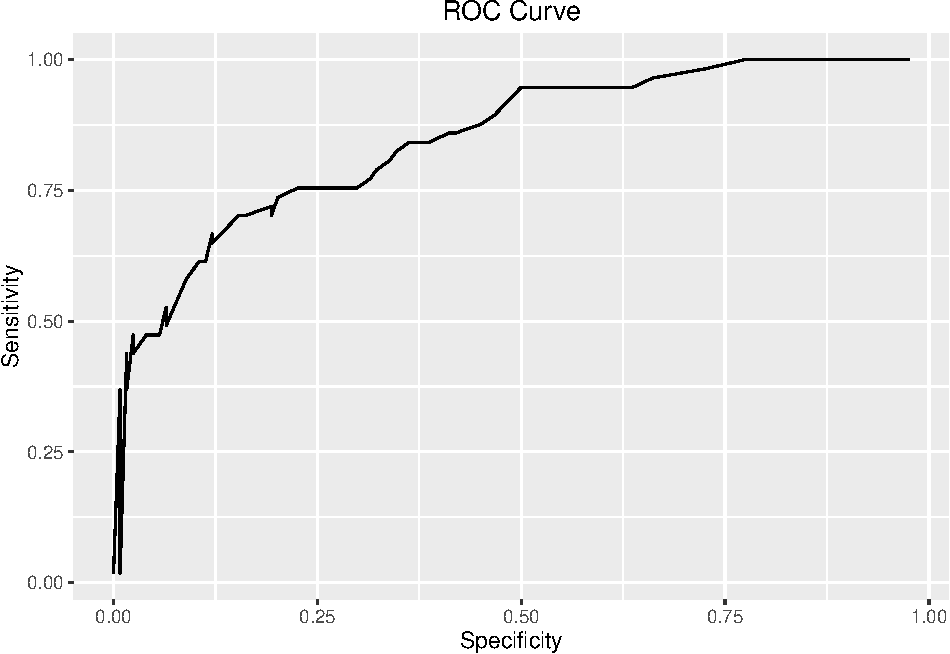
\includegraphics{Week2_yq_files/figure-latex/unnamed-chunk-9-1.pdf}

\begin{Shaded}
\begin{Highlighting}[]
\NormalTok{result$AUC}
\end{Highlighting}
\end{Shaded}

\begin{verbatim}
## [1] 0.8247029
\end{verbatim}

\subsubsection{11. Use your created R functions and the provided
classification output data set to produce all of the classification
metrics discussed
above.}\label{use-your-created-r-functions-and-the-provided-classification-output-data-set-to-produce-all-of-the-classification-metrics-discussed-above.}

\begin{Shaded}
\begin{Highlighting}[]
\KeywordTok{my_accuracy}\NormalTok{(data)}
\end{Highlighting}
\end{Shaded}

\begin{verbatim}
## [1] 0.8066298
\end{verbatim}

\begin{Shaded}
\begin{Highlighting}[]
\KeywordTok{my_error}\NormalTok{(data)}
\end{Highlighting}
\end{Shaded}

\begin{verbatim}
## [1] 0.1933702
\end{verbatim}

\begin{Shaded}
\begin{Highlighting}[]
\KeywordTok{my_precision}\NormalTok{(data)}
\end{Highlighting}
\end{Shaded}

\begin{verbatim}
## [1] 0.84375
\end{verbatim}

\begin{Shaded}
\begin{Highlighting}[]
\KeywordTok{my_sensitivity}\NormalTok{(data)}
\end{Highlighting}
\end{Shaded}

\begin{verbatim}
## [1] 0.4736842
\end{verbatim}

\begin{Shaded}
\begin{Highlighting}[]
\KeywordTok{my_specificity}\NormalTok{(data)}
\end{Highlighting}
\end{Shaded}

\begin{verbatim}
## [1] 0.9596774
\end{verbatim}

\begin{Shaded}
\begin{Highlighting}[]
\KeywordTok{my_f1s}\NormalTok{(data)}
\end{Highlighting}
\end{Shaded}

\begin{verbatim}
## [1] 0.6067416
\end{verbatim}

\subsubsection{12. nvestigate the caret package. In particular, consider
the functions confusionMatrix, sensitivity, and specificity. Apply the
functions to the data
set.}\label{nvestigate-the-caret-package.-in-particular-consider-the-functions-confusionmatrix-sensitivity-and-specificity.-apply-the-functions-to-the-data-set.}

\begin{Shaded}
\begin{Highlighting}[]
\KeywordTok{library}\NormalTok{(caret)}
\end{Highlighting}
\end{Shaded}

\begin{verbatim}
## Warning: package 'caret' was built under R version 3.2.5
\end{verbatim}

\begin{verbatim}
## Loading required package: lattice
\end{verbatim}

\begin{Shaded}
\begin{Highlighting}[]
\KeywordTok{confusionMatrix}\NormalTok{(data$scored.class, data$class, }\DataTypeTok{positive =} \StringTok{"1"}\NormalTok{)}
\end{Highlighting}
\end{Shaded}

\begin{verbatim}
## Confusion Matrix and Statistics
## 
##           Reference
## Prediction   0   1
##          0 119  30
##          1   5  27
##                                           
##                Accuracy : 0.8066          
##                  95% CI : (0.7415, 0.8615)
##     No Information Rate : 0.6851          
##     P-Value [Acc > NIR] : 0.0001712       
##                                           
##                   Kappa : 0.4916          
##  Mcnemar's Test P-Value : 4.976e-05       
##                                           
##             Sensitivity : 0.4737          
##             Specificity : 0.9597          
##          Pos Pred Value : 0.8438          
##          Neg Pred Value : 0.7987          
##              Prevalence : 0.3149          
##          Detection Rate : 0.1492          
##    Detection Prevalence : 0.1768          
##       Balanced Accuracy : 0.7167          
##                                           
##        'Positive' Class : 1               
## 
\end{verbatim}

I got the same accuracy, sensitivity and specificity.

\subsubsection{13. Investigate the pROC package. Use it to generate an
ROC curve for the data set. How do the results compare with your own
functions?}\label{investigate-the-proc-package.-use-it-to-generate-an-roc-curve-for-the-data-set.-how-do-the-results-compare-with-your-own-functions}

\begin{Shaded}
\begin{Highlighting}[]
\KeywordTok{library}\NormalTok{(pROC)}
\end{Highlighting}
\end{Shaded}

\begin{verbatim}
## Type 'citation("pROC")' for a citation.
\end{verbatim}

\begin{verbatim}
## 
## Attaching package: 'pROC'
\end{verbatim}

\begin{verbatim}
## The following objects are masked from 'package:stats':
## 
##     cov, smooth, var
\end{verbatim}

\begin{Shaded}
\begin{Highlighting}[]
\NormalTok{rc <-}\StringTok{ }\KeywordTok{roc}\NormalTok{(}\KeywordTok{as.factor}\NormalTok{(data$class) ~}\StringTok{ }\NormalTok{data$scored.probability)}
\KeywordTok{plot}\NormalTok{(rc,}\DataTypeTok{main=}\StringTok{'ROC Curve'}\NormalTok{)}
\end{Highlighting}
\end{Shaded}

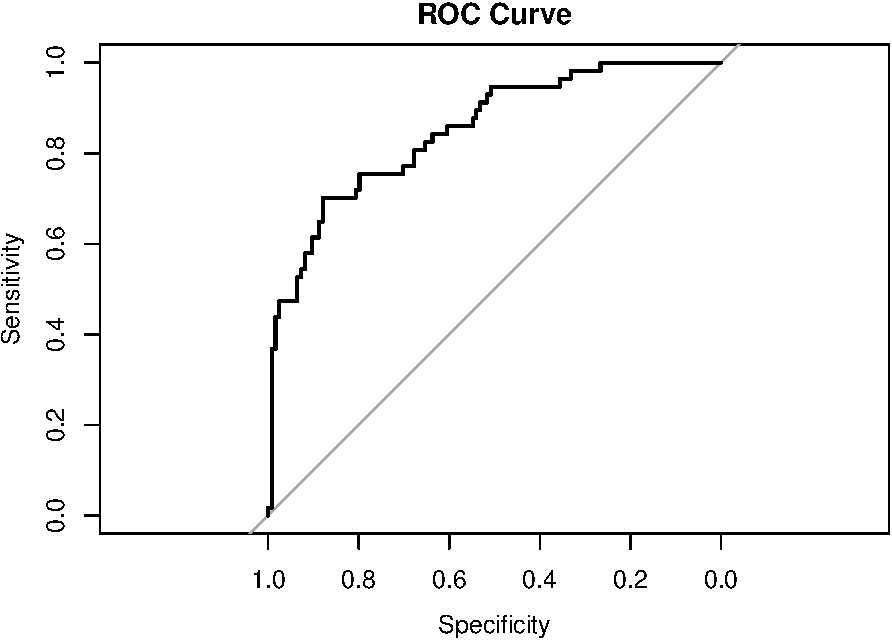
\includegraphics{Week2_yq_files/figure-latex/unnamed-chunk-12-1.pdf}

\begin{verbatim}
## 
## Call:
## roc.formula(formula = as.factor(data$class) ~ data$scored.probability)
## 
## Data: data$scored.probability in 124 controls (as.factor(data$class) 0) < 57 cases (as.factor(data$class) 1).
## Area under the curve: 0.8503
\end{verbatim}

\begin{Shaded}
\begin{Highlighting}[]
\NormalTok{rc$auc}
\end{Highlighting}
\end{Shaded}

\begin{verbatim}
## Area under the curve: 0.8503
\end{verbatim}

\begin{itemize}
\tightlist
\item
  I got the similar curve and the area under the curve.
\end{itemize}

\end{document}
